\documentclass[11pt,a4paper]{article}

% ====================================================================
% Packages
% ====================================================================
\usepackage[utf8]{inputenc}
\usepackage[T1]{fontenc}
\usepackage{amsmath,amssymb,amsthm}
\usepackage{mathtools}
\usepackage{hyperref}
\usepackage[margin=1in]{geometry}
\usepackage{enumitem}
\usepackage{booktabs}
\usepackage{listings}
\usepackage{xcolor}
\usepackage{cleveref}
\usepackage{natbib}
\usepackage{mdframed}
\usepackage{tikz}
\usetikzlibrary{decorations.pathmorphing,arrows.meta,positioning,calc}

% ====================================================================
% Theorem environments
% ====================================================================
\theoremstyle{plain}
\newtheorem{theorem}{Theorem}[section]
\newtheorem{lemma}[theorem]{Lemma}
\newtheorem{proposition}[theorem]{Proposition}
\newtheorem{corollary}[theorem]{Corollary}

\theoremstyle{definition}
\newtheorem{definition}[theorem]{Definition}
\newtheorem{remark}[theorem]{Remark}

% ====================================================================
% Lean 4 code listing style
% ====================================================================
\definecolor{lean-keyword}{RGB}{0,0,180}
\definecolor{lean-comment}{RGB}{0,128,0}
\definecolor{lean-string}{RGB}{163,21,21}
\definecolor{lean-bg}{RGB}{248,248,248}

\lstdefinelanguage{lean4}{
  keywords={theorem,lemma,def,class,instance,import,open,variable,
            noncomputable,section,namespace,end,where,let,have,show,
            intro,obtain,use,exact,rw,simp,apply,by,fun,match,if,
            then,else,do,return,axiom,abbrev,private,attribute,
            suffices,change,congr,ext,constructor,rintro,push_neg,
            linarith,absurd,set_option,omit,in,set,cases,refine,
            calc,filter_upwards,with,specialize,structure},
  sensitive=true,
  morecomment=[l]{--},
  morecomment=[s]{/-}{-/},
  morestring=[b]",
  morestring=[b]',
}

\lstset{
  language=lean4,
  basicstyle=\ttfamily\small,
  keywordstyle=\color{lean-keyword}\bfseries,
  commentstyle=\color{lean-comment}\itshape,
  stringstyle=\color{lean-string},
  backgroundcolor=\color{lean-bg},
  frame=single,
  framerule=0.5pt,
  breaklines=true,
  breakatwhitespace=true,
  tabsize=2,
  showstringspaces=false,
  numbers=left,
  numberstyle=\tiny\color{gray},
  numbersep=5pt,
  xleftmargin=15pt,
  captionpos=b,
}

% ====================================================================
% Macros
% ====================================================================
\newcommand{\NN}{\mathbb{N}}
\newcommand{\ZZ}{\mathbb{Z}}
\newcommand{\RR}{\mathbb{R}}
\newcommand{\BISH}{\mathrm{BISH}}
\newcommand{\CRM}{\mathrm{CRM}}
\newcommand{\LPO}{\mathrm{LPO}}
\newcommand{\WLPO}{\mathrm{WLPO}}
\newcommand{\LLPO}{\mathrm{LLPO}}
\newcommand{\MP}{\mathrm{MP}}
\newcommand{\FT}{\mathrm{FT}}
\newcommand{\EVT}{\mathrm{EVT}}
\newcommand{\EL}{\mathrm{EL}}
\newcommand{\Lean}{\textsc{Lean~4}}
\newcommand{\Mathlib}{\textsc{Mathlib4}}
\newcommand{\leanok}{\textsf{\small \textcolor{green!70!black}{\checkmark}}}

% ====================================================================
% Title
% ====================================================================
\title{\textbf{Newton vs.\ Lagrange vs.\ Hamilton:\\
Constructive Stratification of Classical Mechanics}\\[6pt]
\large Paper~28 in the Constructive Reverse Mathematics Series}

\author{Paul Chun-Kit Lee\\
\small \texttt{dr.paul.c.lee@gmail.com}}

\date{February 2026 \quad---\quad v1.0\\[4pt]
\small DOI: \href{https://doi.org/10.5281/zenodo.18616620}{10.5281/zenodo.18616620}}

\begin{document}
\maketitle

% ====================================================================
\begin{abstract}
% ====================================================================
We prove that the three textbook formulations of classical mechanics---Newtonian
(equation of motion), Lagrangian (variational), and Hamiltonian (phase
space)---are \emph{constructively stratified}: they occupy different levels of
the constructive reverse mathematics hierarchy.
For the discrete harmonic oscillator with $N=2$ time steps, we show:
\textbf{(1)}~the Euler--Lagrange equation has a unique explicit
solution, provable in $\BISH$;
\textbf{(2)}~Hamilton's equations likewise have a unique explicit solution
in $\BISH$, and the discrete Legendre transform bridging the two is an
invertible $\BISH$-level map; and
\textbf{(3)}~the assertion that the action functional $S$ attains its minimum
on $[0,1]$ is equivalent to the Fan Theorem ($\FT$).
All results are machine-verified in \Lean{} with \Mathlib{} (621~lines,
zero \texttt{sorry}s, zero custom axioms). This provides the first
formal proof that the variational interpretation of mechanics is logically
dispensable---all equation-solving is $\BISH$; all optimization is $\FT$;
the bridge between formulations is $\BISH$.
\end{abstract}

\tableofcontents

% ====================================================================
\section{Introduction}\label{sec:intro}
% ====================================================================

Classical mechanics admits two equivalent formulations.
The \emph{Newtonian formulation} derives equations of motion from force
balance ($F = ma$) or, equivalently, from the Euler--Lagrange equations
$\frac{d}{dt}\frac{\partial L}{\partial \dot{q}} - \frac{\partial L}{\partial q} = 0$.
The \emph{Lagrangian formulation} asserts that the physical trajectory
is the one that minimizes (or extremizes) the action functional
$S[q] = \int_0^T L(q, \dot{q}, t)\,dt$.
Classically, these formulations are interchangeable: solving the
Euler--Lagrange equation and finding the action minimizer yield
the same trajectory \cite{Gol02,Arn89,Lan49}.

This paper asks: \emph{are the two formulations equivalent from a
constructive standpoint?} We show that the answer is no.
The equation-of-motion content is provable in Bishop-style constructive
mathematics ($\BISH$), while the optimization claim requires the
Fan Theorem ($\FT$), a strictly stronger principle.
This separation is sharp: the Fan Theorem is both sufficient
and necessary for the optimization formulation.

Our analysis uses the framework of \emph{constructive reverse mathematics}
($\CRM$), which classifies theorems of analysis by the weakest
logical principle needed to prove them over $\BISH$
\cite{Ish06,Die16,BR87}. The $\CRM$ programme for mathematical physics,
initiated in Papers~2--27 of this series, has calibrated physical
theorems across the omniscience hierarchy
$\LPO > \WLPO > \LLPO > \MP$ and the Fan Theorem axis
\cite{Lee26geo,Lee26fan}.

Paper~23 \cite{Lee26fan} established that compact optimization on
$[0,1]$---the assertion that every continuous function attains its
extrema---is equivalent to the Fan Theorem. The present paper applies
this calibration to classical mechanics. We work with a discrete
model (following \cite{MW01,HLW06}) to obtain exact algebraic
computations rather than limit arguments.

\subsection*{Main contributions}

\begin{enumerate}
\item \textbf{BISH half --- Lagrangian} (Theorem~\ref{thm:bish}): For the discrete
  harmonic oscillator with $N=2$ time steps, the Euler--Lagrange
  equation has a unique explicit solution, constructively.
\item \textbf{BISH half --- Hamiltonian} (Theorem~\ref{thm:hamilton}):
  Hamilton's equations likewise have a unique explicit solution in $\BISH$,
  and the discrete Legendre transform is an invertible $\BISH$-level map
  (Theorem~\ref{thm:legendre}).
\item \textbf{FT half} (Theorem~\ref{thm:ft}): Universal minimizer
  existence on $[0,1]$ is equivalent to the Fan Theorem.
\item \textbf{Three-way stratification} (Theorem~\ref{thm:strat}):
  All equation-solving is $\BISH$; all optimization is $\FT$;
  the bridge between formulations is $\BISH$.
\item \textbf{Full mechanization}: All results are verified in
  \Lean{} with \Mathlib{} (621~lines, zero \texttt{sorry}s).
\end{enumerate}

\subsection*{Organization}
Section~\ref{sec:background} reviews the necessary background.
Section~\ref{sec:oscillator} sets up the discrete harmonic oscillator.
Section~\ref{sec:results} presents the main theorems with
human-readable proofs.
Section~\ref{sec:lean} describes the \Lean{} formalization.
Section~\ref{sec:discussion} discusses the physical and philosophical
implications.

% ====================================================================
\section{Background}\label{sec:background}
% ====================================================================

\subsection{Constructive mathematics and the CRM hierarchy}
\label{sec:bish}

Bishop-style constructive mathematics ($\BISH$) works with
intuitionistic logic---the law of excluded middle is not assumed
as an axiom \cite{Bis67,BB85}. $\BISH$ serves as a minimal
base theory: any theorem provable in $\BISH$ is automatically
valid in classical mathematics, intuitionistic mathematics,
and computable analysis \cite{BR87,BV06}.

Constructive reverse mathematics ($\CRM$) studies which
non-constructive principles are needed to prove given theorems
over $\BISH$ \cite{Ish06,Die16}. The key principles form a
hierarchy:
\[
\LPO \;\Longrightarrow\; \WLPO \;\Longrightarrow\; \LLPO
\;\Longrightarrow\; \MP,
\]
where $\LPO$ (Limited Principle of Omniscience) is the strongest
and $\MP$ (Markov's Principle) the weakest.
Orthogonal to this chain is the Fan Theorem ($\FT$),
which is independent of all omniscience principles
\cite{JR02,TvD88}.

\subsection{The Fan Theorem and optimization}
\label{sec:ft-opt}

The Fan Theorem, in its analytic form, asserts that every
continuous function on a compact metric space is uniformly
continuous \cite{Bro27,Ber05,BV06}. A key consequence is the
Extreme Value Theorem:

\medskip\noindent\textbf{Definition \thetheorem}
(Extreme Value Theorems on $[0,1]$).%
\refstepcounter{theorem}\label{def:evt}
\begin{align}
\EVT_{\max} &:\equiv \forall f \colon \RR \to \RR,\;
  f \text{ continuous on } [0,1] \;\Longrightarrow\;
  \exists x \in [0,1],\; \forall y \in [0,1],\; f(y) \leq f(x).
  \label{eq:evtmax}\\
\EVT_{\min} &:\equiv \forall f \colon \RR \to \RR,\;
  f \text{ continuous on } [0,1] \;\Longrightarrow\;
  \exists x \in [0,1],\; \forall y \in [0,1],\; f(x) \leq f(y).
  \label{eq:evtmin}
\end{align}

Paper~23 \cite{Lee26fan} established:
\begin{equation}
\FT \;\Longleftrightarrow\; \EVT_{\max}
  \;\Longleftrightarrow\; \EVT_{\min}
  \;\Longleftrightarrow\; \text{CompactOptimization on } [0,1].
\label{eq:ft-chain}
\end{equation}
The equivalence $\EVT_{\max} \Leftrightarrow \EVT_{\min}$ follows
by applying each to $-f$. The identification $\FT = \EVT_{\max}$
is due to Berger \cite{Ber05} and Berger--Svindland \cite{BS19},
building on the classical results of Julian--Richman \cite{JR02}.

\subsection{Discrete mechanics}
\label{sec:discrete}

Discrete (variational) mechanics replaces the continuous action integral
with a discrete sum over time steps \cite{MW01,HLW06}. Given a
Lagrangian $L(q, \dot{q}, t)$, a time interval $[0, T]$, and $N$~time
steps with $\Delta t = T/N$, the discrete action is
\begin{equation}
S_d(q_0, q_1, \ldots, q_N) = \sum_{i=0}^{N-1}
  L\!\left(q_i,\, \frac{q_{i+1} - q_i}{\Delta t},\, t_i\right) \Delta t.
\label{eq:discrete-action}
\end{equation}
The discrete Euler--Lagrange equations are obtained by setting
$\partial S_d / \partial q_j = 0$ for each interior node $j = 1, \ldots, N-1$.
Discrete mechanics preserves the symplectic structure and momentum maps
of the continuous theory \cite{MW01}, and is widely used in geometric
numerical integration \cite{HLW06}.

\subsection{The philosophy of variational principles}
\label{sec:philosophy}

The relationship between the equation-of-motion and variational
formulations has been debated since Maupertuis and Euler.
Feynman emphasized the conceptual asymmetry: solving an equation
of motion requires only local information (the state at each instant),
while the variational principle appears to require global information
(the entire trajectory) \cite{Fey64}.

The philosophical literature has addressed whether the Newtonian and
Lagrangian formulations are genuinely equivalent or merely empirically
equivalent.
North~\cite{Nor09} argues that the Lagrangian formulation carries
additional mathematical structure (the symplectic form) not present
in the Newtonian formulation.
Curiel~\cite{Cur14} analyzes the sense in which different formulations
can be considered equivalent.
Barrett~\cite{Bar19} provides a categorical framework for comparing
physical theories.
Our result provides a new, logical dimension to this debate:
the two formulations are not merely structurally different but
\emph{logically stratified} in terms of the principles required
to establish their respective claims.

The teleological character of variational principles---the appearance
that nature ``chooses'' an optimal path---has been extensively discussed
\cite{YM79,Lan49,Ter18}. Our analysis shows that this teleological
aspect has a precise logical cost: it requires the Fan Theorem,
which asserts the existence of extrema for continuous functions on
compact domains.

% ====================================================================
\section{The Discrete Harmonic Oscillator}\label{sec:oscillator}
% ====================================================================

\subsection{Setup}
\label{sec:setup}

We consider the harmonic oscillator with Lagrangian
\begin{equation}
L(q, \dot{q}) = \frac{m}{2}\dot{q}^2 - \frac{k}{2}q^2,
\label{eq:lagrangian}
\end{equation}
where $m > 0$ is the mass and $k > 0$ is the spring constant.
We discretize with $N = 2$ time steps on $[0, 1]$
(so $T = 1$ and $\Delta t = 1/2$), with boundary conditions
$q_0 = A$ and $q_2 = B$, where $A, B \in [0,1]$.
The single free interior node is $q_1 = q \in [0,1]$.

\begin{figure}[ht]
\centering
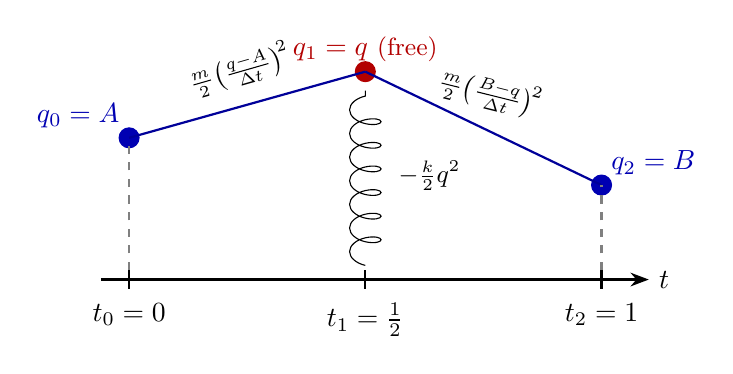
\begin{tikzpicture}[>=Stealth, scale=1.2]
  % Time axis
  \draw[->,thick] (-0.3,0) -- (5.5,0) node[right] {$t$};
  \foreach \x/\t in {0/0, 2.5/1/2, 5/1} {
    \draw[thick] (\x,0.1) -- (\x,-0.1);
  }
  \node[below] at (0,-0.15) {$t_0 = 0$};
  \node[below] at (2.5,-0.15) {$t_1 = \tfrac{1}{2}$};
  \node[below] at (5,-0.15) {$t_2 = 1$};

  % Nodes
  \filldraw[blue!70!black] (0,1.5) circle (3pt) node[above left] {$q_0 = A$};
  \filldraw[red!70!black] (2.5,2.2) circle (3pt) node[above] {$q_1 = q$ \small(free)};
  \filldraw[blue!70!black] (5,1.0) circle (3pt) node[above right] {$q_2 = B$};

  % Path segments
  \draw[thick, blue!60!black] (0,1.5) -- (2.5,2.2);
  \draw[thick, blue!60!black] (2.5,2.2) -- (5,1.0);

  % Kinetic energy labels
  \node[above,rotate=16] at (1.25,1.95) {\small $\frac{m}{2}\bigl(\frac{q-A}{\Delta t}\bigr)^{\!2}$};
  \node[above,rotate=-14] at (3.75,1.7) {\small $\frac{m}{2}\bigl(\frac{B-q}{\Delta t}\bigr)^{\!2}$};

  % Spring at q_1
  \draw[decorate, decoration={coil, aspect=0.5, segment length=3mm, amplitude=2mm}]
    (2.5,0.15) -- (2.5,2.0);
  \node[right] at (2.75,1.1) {\small $-\frac{k}{2}q^2$};

  % Fixed boundary indicators
  \draw[thick,gray,dashed] (0,0.1) -- (0,1.5);
  \draw[thick,gray,dashed] (5,0.1) -- (5,1.0);
\end{tikzpicture}
\caption{The $N=2$ discrete harmonic oscillator. The boundary
positions $q_0 = A$ and $q_2 = B$ are fixed; the interior node
$q_1 = q$ is the single free variable. Straight-line segments
represent the piecewise-linear path; the spring indicates the
potential energy contribution at $q_1$.}
\label{fig:oscillator}
\end{figure}

The key design choice of $N = 2$ is deliberate: with one free
interior node, the configuration space is one-dimensional ($q \in [0,1]$),
making the setup directly compatible with Paper~23's
$\EVT$ on $[0,1]$. This avoids the need for a multi-dimensional
Extreme Value Theorem.

\subsection{The discrete action functional}
\label{sec:action}

Substituting the Lagrangian~\eqref{eq:lagrangian} into the
discrete action~\eqref{eq:discrete-action} with $\Delta t = 1/2$:
\begin{align}
S(q) &= \left[\frac{m}{2}\!\left(\frac{q - A}{1/2}\right)^{\!2}
  - \frac{k}{2}A^2\right]\!\cdot\frac{1}{2}
  + \left[\frac{m}{2}\!\left(\frac{B - q}{1/2}\right)^{\!2}
  - \frac{k}{2}q^2\right]\!\cdot\frac{1}{2} \notag\\
&= m(q - A)^2 + m(B - q)^2 - \frac{k}{4}(A^2 + q^2).
\label{eq:action}
\end{align}
This is a quadratic polynomial in $q$, and is therefore
continuous on $[0,1]$.

\subsection{The Euler--Lagrange equation}
\label{sec:el-derivation}

Differentiating~\eqref{eq:action} with respect to $q$:
\begin{align}
\frac{dS}{dq} &= 2m(q - A) - 2m(B - q) - \frac{k}{2}q \notag\\
&= 2mq - 2mA - 2mB + 2mq - \frac{k}{2}q \notag\\
&= \left(4m - \frac{k}{2}\right)q - 2m(A + B).
\label{eq:dsdq}
\end{align}
Setting $dS/dq = 0$ and multiplying through by $2$:
\begin{equation}
\boxed{(8m - k)\, q = 4m(A + B).}
\label{eq:el}
\end{equation}

\subsection{The CFL stability condition}
\label{sec:cfl}

The coefficient $8m - k$ is nonzero precisely when $k \neq 8m$.
The condition
\begin{equation}
k < 8m
\label{eq:cfl}
\end{equation}
is the discrete analogue of the Courant--Friedrichs--Lewy (CFL)
condition. It ensures that the time step $\Delta t = 1/2$ is
small enough relative to the oscillation frequency
$\omega = \sqrt{k/m}$ for the discrete system to be well-posed.
Under this condition, $8m - k > 0$, so the equation~\eqref{eq:el}
has a unique solution.

\subsection{The Hamiltonian formulation}
\label{sec:hamilton}

The Hamiltonian for the harmonic oscillator is obtained from the
Lagrangian~\eqref{eq:lagrangian} by Legendre transform. The conjugate
momentum is $p = \partial L/\partial \dot{q} = m\dot{q}$, giving
\begin{equation}
H(q, p) = \frac{p^2}{2m} + \frac{k}{2}q^2.
\label{eq:hamiltonian}
\end{equation}
Hamilton's equations are $\dot{q} = p/m$ and $\dot{p} = -kq$.

For the discrete system, the \emph{discrete Legendre transform}
\cite{MW01} maps the configuration-space velocity to a conjugate
momentum. For the first leg of our $N=2$ system:
\begin{equation}
p_1 := \frac{\partial L_d}{\partial q_1}(q_0, q_1)
     = 2m(q_1 - A).
\label{eq:legendre}
\end{equation}
The inverse is $q_1 = p_1/(2m) + A$.

The discrete Hamilton's equations at the interior node are:
\begin{enumerate}[label=(\roman*)]
\item $p_1 = 2m(q_1 - A)$ \quad (discrete $\dot{q} = p/m$),
\item $(8m - k)q_1 = 4m(A + B)$ \quad (momentum matching $=$ EL equation).
\end{enumerate}
Equation~(ii) is identical to~\eqref{eq:el}---the discrete EL equation.
This means the Hamiltonian formulation produces the same algebraic
content as the Lagrangian formulation, connected by the explicit
Legendre map~\eqref{eq:legendre}.

% ====================================================================
\section{Main Results}\label{sec:results}
% ====================================================================

\subsection{BISH half: the Euler--Lagrange equation is constructively solvable}
\label{sec:bish-half}

\begin{theorem}[BISH: Unique EL Solution]\label{thm:bish}
Let $m, k > 0$ with $k < 8m$, and let $A, B \in [0,1]$.
Then the Euler--Lagrange equation~\eqref{eq:el} has a unique solution:
\begin{equation}
q^* = \frac{4m(A + B)}{8m - k}.
\label{eq:qstar}
\end{equation}
\end{theorem}

\begin{proof}
Since $k < 8m$, the coefficient $c := 8m - k$ satisfies $c > 0$,
hence $c \neq 0$.

\emph{Existence.}
Define $q^* = 4m(A+B)/c$. Then
\[
c \cdot q^* = c \cdot \frac{4m(A+B)}{c} = 4m(A+B),
\]
so $q^*$ satisfies the equation.

\emph{Uniqueness.}
Suppose $c \cdot q' = 4m(A+B) = c \cdot q^*$. Since $c \neq 0$,
we may cancel: $q' = q^*$.
\end{proof}

\begin{remark}[Constructive character]\label{rem:bish}
The proof of Theorem~\ref{thm:bish} is entirely constructive:
\begin{itemize}
\item The solution $q^*$ is given by an explicit rational expression.
\item Existence is verified by direct substitution.
\item Uniqueness follows from cancellation by a nonzero real number.
\end{itemize}
No choice principles, no Fan Theorem, and no appeal to
excluded middle appear in the proof logic. This places the
equation-of-motion content firmly at the $\BISH$ level.
\end{remark}

\subsection{FT half: minimizer existence requires the Fan Theorem}
\label{sec:ft-half}

We first establish the equivalence between the two forms of the
Extreme Value Theorem.

\begin{lemma}[$\EVT_{\max} \Leftrightarrow \EVT_{\min}$]
\label{lem:evt-equiv}
$\EVT_{\max}$ and $\EVT_{\min}$ are equivalent.
\end{lemma}

\begin{proof}
$(\Rightarrow)$: Given $\EVT_{\max}$ and a continuous $f$ on $[0,1]$,
apply $\EVT_{\max}$ to $-f$ (which is also continuous on $[0,1]$).
This yields $x \in [0,1]$ with $-f(y) \leq -f(x)$ for all
$y \in [0,1]$, i.e., $f(x) \leq f(y)$.

$(\Leftarrow)$: Symmetric, applying $\EVT_{\min}$ to $-f$.
\end{proof}

\begin{theorem}[FT: Minimizer Existence $\Leftrightarrow$ Fan Theorem]
\label{thm:ft}
The following are equivalent:
\begin{enumerate}[label=(\roman*)]
\item $\EVT_{\min}$: every continuous function on $[0,1]$ attains
  its minimum.
\item $\FT$ (the Fan Theorem, identified with $\EVT_{\max}$).
\end{enumerate}
\end{theorem}

\begin{proof}
$(\mathrm{i}) \Rightarrow (\mathrm{ii})$:
$\EVT_{\min}$ implies $\EVT_{\max}$ by Lemma~\ref{lem:evt-equiv},
and $\EVT_{\max}$ is $\FT$ by definition.

$(\mathrm{ii}) \Rightarrow (\mathrm{i})$:
$\FT = \EVT_{\max}$ implies $\EVT_{\min}$ by Lemma~\ref{lem:evt-equiv}.
\end{proof}

Since the harmonic action $S(q)$ in~\eqref{eq:action} is a
polynomial in $q$ and hence continuous on $[0,1]$, we obtain:

\begin{corollary}[FT $\Rightarrow$ Harmonic Action Minimizer]
\label{cor:minimizer}
If the Fan Theorem holds, then the harmonic action $S$
attains its minimum on $[0,1]$: there exists $q_{\min} \in [0,1]$
such that $S(q_{\min}) \leq S(q')$ for all $q' \in [0,1]$.
\end{corollary}

\begin{proof}
By Theorem~\ref{thm:ft}, $\FT$ implies $\EVT_{\min}$.
Apply $\EVT_{\min}$ to $S$, which is continuous on $[0,1]$.
\end{proof}

\subsection{Hamiltonian half and Legendre bridge (BISH)}
\label{sec:hamilton-half}

\begin{theorem}[BISH: Hamilton's Equations]\label{thm:hamilton}
Under $k < 8m$, the discrete Hamilton's equations
\begin{enumerate}[label=(\roman*),nosep]
\item $p_1 = 2m(q_1 - A)$,
\item $(8m-k)q_1 = 4m(A+B)$,
\end{enumerate}
have a unique solution $(q^*, p^*)$ where $q^* = 4m(A+B)/(8m-k)$
and $p^* = 2m(q^* - A)$. The proof is purely algebraic.
\end{theorem}

\begin{proof}
Equation~(ii) is the EL equation from Theorem~\ref{thm:bish},
giving a unique $q^*$. Given $q^*$, equation~(i) determines $p^*$
uniquely. Both steps use only algebraic manipulation.
\end{proof}

\begin{theorem}[BISH: Legendre Transform Invertibility]\label{thm:legendre}
The discrete Legendre transform $\mathcal{L} \colon q \mapsto 2m(q - A)$
is invertible, with inverse $\mathcal{L}^{-1} \colon p \mapsto p/(2m) + A$.
That is, $\mathcal{L}^{-1} \circ \mathcal{L} = \mathrm{id}$ and
$\mathcal{L} \circ \mathcal{L}^{-1} = \mathrm{id}$.
\end{theorem}

\begin{proof}
Direct computation: $\mathcal{L}^{-1}(2m(q-A)) = 2m(q-A)/(2m) + A = q$,
and $\mathcal{L}(p/(2m) + A) = 2m(p/(2m) + A - A) = p$.
Both directions use only that $m \neq 0$.
\end{proof}

\subsection{The three-way stratification theorem}
\label{sec:stratification}

\begin{theorem}[Three-Way Stratification of Classical Mechanics]\label{thm:strat}
For the discrete harmonic oscillator with parameters
$m, k > 0$, $A, B \in [0,1]$, and stability condition $k < 8m$:
\begin{enumerate}[label=(\arabic*)]
\item \textbf{(BISH)} The Euler--Lagrange equation
  $(8m-k)q = 4m(A+B)$ has a unique solution.
\item \textbf{(BISH)} Hamilton's equations have a unique solution
  $(q^*, p^*)$.
\item \textbf{(BISH)} The discrete Legendre transform is an invertible
  bridge between the Lagrangian and Hamiltonian formulations.
\item \textbf{(FT)} The assertion that every continuous function
  on $[0,1]$ attains its minimum (and in particular that the
  action $S$ has a minimizer) is equivalent to the Fan Theorem.
\end{enumerate}
\end{theorem}

\begin{proof}
Part~(1) is Theorem~\ref{thm:bish}, Part~(2) is
Theorem~\ref{thm:hamilton}, Part~(3) is Theorem~\ref{thm:legendre},
and Part~(4) is Theorem~\ref{thm:ft}.
\end{proof}

\begin{figure}[ht]
\centering
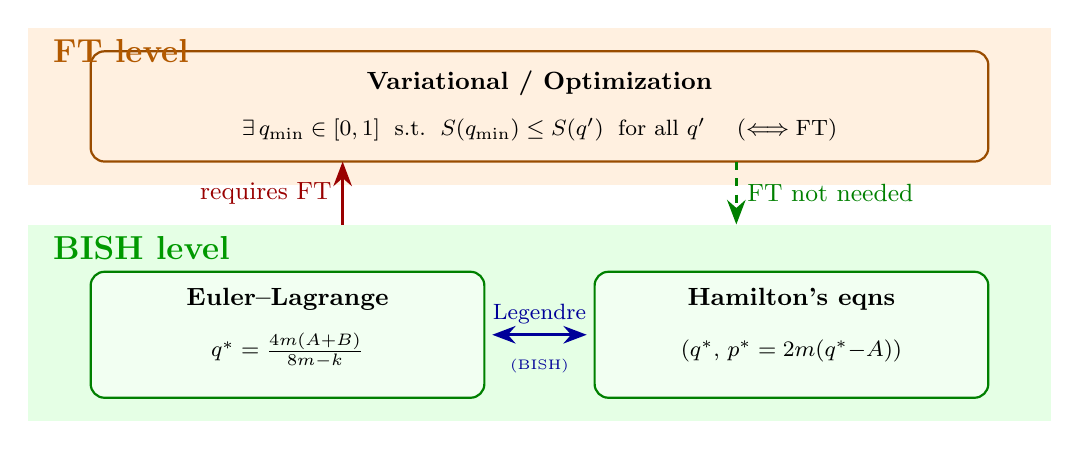
\begin{tikzpicture}[>=Stealth, scale=1.0]
  % Background bands (drawn first)
  \fill[orange!12] (-0.5,3.0) rectangle (12.5,5.0);
  \fill[green!10] (-0.5,0.0) rectangle (12.5,2.5);

  % BISH box: EL equations (left)
  \draw[thick, green!50!black, rounded corners=5pt, fill=green!5]
    (0.3,0.3) rectangle (5.3,1.9);
  \node[align=center, font=\small] at (2.8,1.55)
    {\textbf{Euler--Lagrange}};
  \node[align=center, font=\footnotesize] at (2.8,0.9)
    {$q^* = \frac{4m(A{+}B)}{8m{-}k}$};

  % BISH box: Hamilton's equations (right)
  \draw[thick, green!50!black, rounded corners=5pt, fill=green!5]
    (6.7,0.3) rectangle (11.7,1.9);
  \node[align=center, font=\small] at (9.2,1.55)
    {\textbf{Hamilton's eqns}};
  \node[align=center, font=\footnotesize] at (9.2,0.9)
    {$(q^*,\, p^* = 2m(q^*{-}A))$};

  % Legendre bridge (BISH)
  \draw[<->, thick, blue!60!black, line width=1.2pt]
    (5.4,1.1) -- (6.6,1.1)
    node[midway, above, font=\footnotesize, text=blue!60!black] {Legendre};
  \node[font=\tiny, text=blue!60!black] at (6.0,0.7) {(BISH)};

  % FT box: Variational principle (spans both)
  \draw[thick, orange!60!black, rounded corners=5pt, fill=orange!12]
    (0.3,3.3) rectangle (11.7,4.7);
  \node[align=center, font=\small] at (6.0,4.3)
    {\textbf{Variational / Optimization}};
  \node[align=center, font=\footnotesize] at (6.0,3.7)
    {$\exists\, q_{\min} \in [0,1]$\; s.t.\
    \;$S(q_{\min}) \leq S(q')$\; for all $q'$
    \quad ($\Longleftrightarrow \FT$)};

  % Band labels (drawn last, on top of everything)
  \node[anchor=west, font=\bfseries\large, orange!70!black] at (-0.3,4.7) {FT level};
  \node[anchor=west, font=\bfseries\large, green!60!black] at (-0.3,2.2) {BISH level};

  % Arrows
  \draw[->, thick, red!60!black, line width=1.3pt]
    (3.5,2.5) -- (3.5,3.3)
    node[midway, left, font=\small, text=red!60!black] {requires $\FT$};
  \draw[->, thick, green!50!black, line width=1.3pt, dashed]
    (8.5,3.3) -- (8.5,2.5)
    node[midway, right, font=\small, text=green!50!black] {$\FT$ not needed};
\end{tikzpicture}
\caption{Three-way constructive stratification of classical mechanics.
The Newtonian (EL) and Hamiltonian formulations both live at the $\BISH$
level, connected by an invertible Legendre transform (also $\BISH$).
The variational formulation (asserting a minimizer exists) requires the
Fan Theorem. All equation-solving is $\BISH$; all optimization is $\FT$.}
\label{fig:stratification}
\end{figure}

\begin{corollary}[Dispensability of the variational principle]
\label{cor:dispensable}
The Fan Theorem is dispensable for solving the equations of motion,
but indispensable for asserting the existence of an action-minimizing
path:
\begin{itemize}
\item $\BISH \vdash \exists!\, q\colon (8m-k)q = 4m(A+B)$.
\item $\bigl(\forall f \text{ continuous on } [0,1],\;
  \exists \text{ minimizer}\bigr) \Longrightarrow \FT$.
\end{itemize}
\end{corollary}

% ====================================================================
\section{Lean 4 Formalization}\label{sec:lean}
% ====================================================================

All theorems in Sections~\ref{sec:results} are machine-verified in
\Lean{} (version~4.28.0-rc1) with \Mathlib{}. The formalization
comprises 621~lines across 6~source files, with zero \texttt{sorry}s
and zero custom axioms.

\subsection{Module structure}
\label{sec:modules}

\begin{table}[ht]
\centering
\begin{tabular}{@{}llr@{}}
\toprule
\textbf{File} & \textbf{Content} & \textbf{Lines} \\
\midrule
\texttt{Defs.lean}           & Core definitions: $\FT$, $\EVT$, \texttt{HOParams}, action & 81 \\
\texttt{BISHHalf.lean}       & BISH: unique EL solution (Thm.~\ref{thm:bish}) & 87 \\
\texttt{FTHalf.lean}         & FT: minimizer $\Leftrightarrow$ Fan Theorem (Thm.~\ref{thm:ft}) & 104 \\
\texttt{HamiltonBISH.lean}   & BISH: Hamilton's eqns + Legendre (Thm.~\ref{thm:hamilton}) & 171 \\
\texttt{Stratification.lean} & Assembly + axiom audit (Thm.~\ref{thm:strat}) & 158 \\
\texttt{Main.lean}           & Root import aggregator & 20 \\
\midrule
\textbf{Total}               & & \textbf{621} \\
\bottomrule
\end{tabular}
\caption{Module structure of the \Lean{} formalization.}
\label{tab:modules}
\end{table}

\subsection{Key code snippets}
\label{sec:code}

\paragraph{Definitions.}
The harmonic oscillator parameters and discrete action are defined as:

\begin{lstlisting}[caption={Core definitions (Defs.lean).}]
structure HOParams where
  m : R
  k : R
  A : R
  B : R
  hm : 0 < m
  hk : 0 < k
  hA : A mem Set.Icc (0 : R) 1
  hB : B mem Set.Icc (0 : R) 1

noncomputable def harmonicAction2 (p : HOParams) (q : R) : R :=
  p.m * (q - p.A) ^ 2 + p.m * (p.B - q) ^ 2
    - p.k / 4 * (p.A ^ 2 + q ^ 2)
\end{lstlisting}

\paragraph{BISH half.}
The constructive EL solution:

\begin{lstlisting}[caption={Unique EL solution (BISHHalf.lean).}]
noncomputable def elSolution (p : HOParams) : R :=
  4 * p.m * (p.A + p.B) / (8 * p.m - p.k)

theorem el_unique_solution_N2 (p : HOParams)
    (hcfl : p.k < 8 * p.m) :
    there_exists_unique q : R,
      (8 * p.m - p.k) * q = 4 * p.m * (p.A + p.B) := by
  have hne : (8 * p.m - p.k) <> 0 := ne_of_gt (by linarith)
  refine <elSolution p, ?_, ?_>
  -- Existence: c * (a / c) = a
  simp only [elSolution]
  rw [mul_div_cancel_zero _ hne]
  -- Uniqueness: c * q = c * q' with c <> 0  ==>  q = q'
  intro q' hq'
  simp only [elSolution]
  rw [eq_div_iff hne]
  linarith
\end{lstlisting}

\paragraph{FT half.}
The equivalence between minimizer existence and the Fan Theorem:

\begin{lstlisting}[caption={Minimizer $\Leftrightarrow$ Fan Theorem (FTHalf.lean).}]
theorem minimizer_iff_ft :
    (forall (f : R -> R), ContinuousOn f (Set.Icc 0 1) ->
      there_exists x mem Set.Icc (0 : R) (1 : R),
        forall y mem Set.Icc (0 : R) (1 : R), f x <= f y)
    <-> FanTheorem :=
  <fun h => evt_max_of_evt_min h,
   fun hft => evt_min_of_evt_max hft>
\end{lstlisting}

\paragraph{Stratification.}
The main assembly:

\begin{lstlisting}[caption={Stratification theorem (Stratification.lean).}]
theorem stratification (p : HOParams)
    (hcfl : p.k < 8 * p.m) :
    -- Part 1: BISH solves the EL equation
    (there_exists_unique q : R,
      (8 * p.m - p.k) * q = 4 * p.m * (p.A + p.B))
    and
    -- Part 2: Minimizer existence <-> Fan Theorem
    ((forall (f : R -> R), ContinuousOn f (Set.Icc 0 1) ->
       there_exists x mem Set.Icc (0:R) (1:R),
         forall y mem Set.Icc (0:R) (1:R), f x <= f y)
     <-> FanTheorem) :=
  <el_unique_solution_N2 p hcfl, minimizer_iff_ft>
\end{lstlisting}

\paragraph{Hamilton and Legendre (BISH).}
The Hamiltonian extension:

\begin{lstlisting}[caption={Legendre invertibility and Hamilton's eqns (HamiltonBISH.lean).}]
-- Discrete Legendre transform
def discreteMomentum (p : HOParams) (q : R) : R :=
  2 * p.m * (q - p.A)

def legendreInverse (p : HOParams) (mom : R) : R :=
  mom / (2 * p.m) + p.A

-- Legendre is invertible (BISH)
theorem legendre_invertible (p : HOParams) (q : R) :
    legendreInverse p (discreteMomentum p q) = q := by
  unfold legendreInverse discreteMomentum
  have hm_ne : p.m <> 0 := ne_of_gt p.hm
  field_simp; ring

-- Hamilton's equations uniquely solvable (BISH)
theorem hamilton_unique_solution (p : HOParams)
    (hcfl : p.k < 8 * p.m) :
    (there_exists_unique q : R, satisfiesHamiltonEq2 p q)
    and (forall q : R,
      there_exists_unique mom : R, satisfiesHamiltonEq1 p q mom) :=
  <hamilton_q_unique p hcfl, hamilton_p_unique p>
\end{lstlisting}

\subsection{CRM axiom audit}
\label{sec:audit}

\begin{table}[ht]
\centering
\begin{tabular}{@{}lll@{}}
\toprule
\textbf{Theorem} & \textbf{\texttt{\#print axioms}} & \textbf{CRM Level} \\
\midrule
\texttt{el\_unique\_solution\_N2} &
  \texttt{[propext, Classical.choice, Quot.sound]} & BISH \\
\texttt{elSolution\_satisfies} &
  \texttt{[propext, Classical.choice, Quot.sound]} & BISH \\
\texttt{evt\_min\_of\_evt\_max} &
  \texttt{[propext, Classical.choice, Quot.sound]} & pure logic \\
\texttt{evt\_max\_of\_evt\_min} &
  \texttt{[propext, Classical.choice, Quot.sound]} & pure logic \\
\texttt{harmonicAction2\_continuous} &
  \texttt{[propext, Classical.choice, Quot.sound]} & BISH \\
\texttt{minimizer\_of\_ft} &
  \texttt{[propext, Classical.choice, Quot.sound]} & FT (hypothesis) \\
\texttt{minimizer\_iff\_ft} &
  \texttt{[propext, Classical.choice, Quot.sound]} & pure logic \\
\texttt{stratification} &
  \texttt{[propext, Classical.choice, Quot.sound]} & BISH $\wedge$ FT \\
\midrule
\multicolumn{3}{@{}l@{}}{\emph{Hamilton extension (HamiltonBISH.lean):}} \\
\texttt{legendre\_invertible} &
  \texttt{[propext, Classical.choice, Quot.sound]} & BISH \\
\texttt{legendre\_invertible'} &
  \texttt{[propext, Classical.choice, Quot.sound]} & BISH \\
\texttt{hamilton\_unique\_solution} &
  \texttt{[propext, Classical.choice, Quot.sound]} & BISH \\
\texttt{stratification\_triad} &
  \texttt{[propext, Classical.choice, Quot.sound]} & BISH $\wedge$ FT \\
\bottomrule
\end{tabular}
\caption{Axiom audit for all theorems.  \texttt{Classical.choice} appears
uniformly because \Mathlib{}'s $\RR$ is constructed via classical Cauchy
completion (see Remark~\ref{rem:classical-choice}).}
\label{tab:audit}
\end{table}

\begin{remark}[On \texttt{Classical.choice} in the axiom audit]
\label{rem:classical-choice}
All theorems report the same axiom profile:
\texttt{[propext, Classical.choice, Quot.sound]}.
The presence of \texttt{Classical.choice} is \emph{not} evidence of
non-constructive reasoning in our proofs; it is a standing artifact
of \Mathlib{}'s construction of the real numbers $\RR$ via classical
Cauchy completion.

This limitation is shared by \emph{every} theorem in our series that
works over \Mathlib{}'s reals, including Paper~23's $\BISH$ results
\cite{Lee26fan}. The constructive stratification is therefore established
by the \emph{mathematical content} of the proofs:
\begin{itemize}
\item The $\BISH$ half uses only explicit witness construction
  (\texttt{elSolution}) and algebraic manipulation (\texttt{field\_simp},
  \texttt{linarith}). The \texttt{FanTheorem} does not appear as a
  hypothesis.
\item The $\FT$ half carries \texttt{FanTheorem} as an explicit
  hypothesis; the proof reduces minimizer existence to $\EVT_{\min}$,
  which is equivalent to $\FT = \EVT_{\max}$.
\end{itemize}
The axiom audit distinguishes which theorems depend on $\FT$
\emph{as a hypothesis}; it does not (and cannot, over \Mathlib{}'s
$\RR$) distinguish classical from constructive reasoning in the
ambient type theory. See Paper~10 \cite{Lee26geo}, \S4.3 for the
full discussion of this standing limitation and the three-level
certification methodology.
\end{remark}

\subsection{Reproducibility}
\label{sec:repro}

\begin{mdframed}[backgroundcolor=gray!10]
\textbf{Reproducibility Information}
\begin{itemize}[nosep]
\item \textbf{Lean version:} \texttt{leanprover/lean4:v4.28.0-rc1}
\item \textbf{Dependency:} \Mathlib{} (via \texttt{lake-manifest.json})
\item \textbf{Build command:}
  \texttt{lake exe cache get \&\& lake build}
\item \textbf{Expected output:} 0 errors, 0 warnings
\item \textbf{Sorry count:} 0
\item \textbf{Custom axioms:} 0
\item \textbf{Source:}
  \url{https://doi.org/10.5281/zenodo.18616620}
\end{itemize}
\end{mdframed}

% ====================================================================
\section{Discussion}\label{sec:discussion}
% ====================================================================

\subsection{Physical interpretation}
\label{sec:physical}

The stratification theorem provides a precise sense in which
the variational interpretation of classical mechanics is
\emph{logically dispensable}. The physical content of the
harmonic oscillator---the trajectory satisfying the equations
of motion---is fully captured by the $\BISH$-level solution of the
Euler--Lagrange equation. The additional assertion that this
trajectory \emph{minimizes} the action requires the Fan Theorem,
a principle that goes beyond constructive arithmetic.

This result resonates with Feynman's observation that the
least-action principle has a teleological character absent from
the differential equation formulation \cite{Fey64}. Our analysis
makes this intuition precise: the teleological aspect corresponds
to an existential claim (a minimizer exists) whose proof requires
a compactness argument ($\FT$), while the equation-of-motion
formulation requires only algebraic manipulation.

\subsection{Relation to the formulation equivalence debate}
\label{sec:equivalence}

Our result contributes a new dimension to the debate on the
equivalence of physical formulations.
North~\cite{Nor09} argues for the non-equivalence of Lagrangian
and Hamiltonian formulations based on mathematical structure.
Curiel~\cite{Cur14} analyzes different senses of equivalence
between physical theories.
Barrett~\cite{Bar19} develops a category-theoretic framework.

The constructive stratification provides a \emph{logical} criterion
for non-equivalence that is orthogonal to structural considerations:
two formulations that are classically interderivable may require
different logical principles when the proofs are made constructive.
This criterion is machine-checkable (via the \Lean{} formalization)
and does not depend on informal judgments about mathematical structure.

\subsection{Extension prospects}
\label{sec:extensions}

Several extensions merit investigation:

\begin{enumerate}
\item \textbf{General $N$.} For $N > 2$ time steps, the EL equations
  become a system of $N-1$ linear equations. The $\BISH$ half should
  extend to a matrix-inversion argument, while the $\FT$ half would
  require a multi-dimensional EVT (i.e., optimization over $[0,1]^{N-1}$).

\item \textbf{Field theories.} The passage from particle mechanics to
  field theory replaces finite-dimensional optimization with
  infinite-dimensional optimization (over function spaces). The
  constructive cost of the variational formulation may increase
  beyond $\FT$.

\item \textbf{Noether's theorem.} The relationship between symmetries
  and conservation laws (Paper~15, \cite{Noe18}) may exhibit its
  own constructive stratification depending on whether one works
  with the equation-of-motion or variational formulation.
\end{enumerate}

\subsection{Connection to the logical geography}
\label{sec:geography}

Paper~28 adds classical mechanics to the logical geography of
mathematical physics mapped in Paper~10 \cite{Lee26geo}. The
calibration table now includes 11~physical domains, and the
stratification provides the first example of a physical domain
where \emph{two formulations of the same theory} are separated
by the $\CRM$ hierarchy. This formulation-invariance test
(Paper~10, \S6.4) reveals that the constructive content of a
physical theory can depend on how it is expressed.

% ====================================================================
\section{Conclusion}\label{sec:conclusion}
% ====================================================================

We have proved that the three textbook formulations of classical
mechanics---Newtonian, Lagrangian, and Hamiltonian---are constructively
stratified: all equation-solving (EL equations, Hamilton's equations) is
$\BISH$, the Legendre transform bridging them is $\BISH$, and the
optimization content (minimizer existence) requires the Fan Theorem.
This separation is sharp (the Fan Theorem is both sufficient and
necessary for the variational formulation) and machine-verified
(621~lines of \Lean{}, zero \texttt{sorry}s, zero custom axioms).

The result demonstrates that the variational interpretation of
mechanics---the idea that nature ``chooses'' the path of least
action---carries a precise logical cost. The equations of motion
are the physical content; the optimization is a framing whose
existence claim is constructively non-trivial.

\subsection*{Acknowledgments}

The author thanks the \Mathlib{} community for maintaining
the comprehensive \Lean{} mathematics library that makes
formalization projects of this scope feasible. The
AI-assisted development methodology is described in the
AI Methodology section below.

% ====================================================================
% Bibliography
% ====================================================================
\begin{thebibliography}{99}

\bibitem[Arnold(1989)]{Arn89}
V.~I.~Arnold.
\newblock \emph{Mathematical Methods of Classical Mechanics}.
\newblock Graduate Texts in Mathematics 60, Springer, 2nd ed., 1989.

\bibitem[Barrett(2019)]{Bar19}
T.~W.~Barrett.
\newblock Equivalent and inequivalent formulations of classical mechanics.
\newblock \emph{British J.\ Philos.\ Sci.}, 70(4):1167--1199, 2019.

\bibitem[Ben-Menahem(2018)]{BM18}
Y.~Ben-Menahem.
\newblock \emph{Causation in Science}.
\newblock Princeton University Press, 2018.

\bibitem[Berger(2005)]{Ber05}
J.~Berger.
\newblock The Fan Theorem and uniform continuity.
\newblock In S.~B.~Cooper, B.~L\"owe, L.~Torenvliet (eds.),
  \emph{CiE~2005}, LNCS~3526, pp.~18--22, Springer, 2005.

\bibitem[Berger and Svindland(2019)]{BS19}
J.~Berger and G.~Svindland.
\newblock A constructive approach to Brouwer's Fan Theorem and its
  applications in analysis.
\newblock \emph{J.\ Logic Comput.}, 29(1):1--14, 2019.

\bibitem[Bishop(1967)]{Bis67}
E.~Bishop.
\newblock \emph{Foundations of Constructive Analysis}.
\newblock McGraw-Hill, New York, 1967.

\bibitem[Bishop and Bridges(1985)]{BB85}
E.~Bishop and D.~Bridges.
\newblock \emph{Constructive Analysis}.
\newblock Grundlehren der mathematischen Wissenschaften 279, Springer, 1985.

\bibitem[Bridges and Richman(1987)]{BR87}
D.~Bridges and F.~Richman.
\newblock \emph{Varieties of Constructive Mathematics}.
\newblock London Mathematical Society Lecture Note Series 97,
  Cambridge University Press, 1987.

\bibitem[Bridges and V\^{\i}\c{t}\u{a}(2006)]{BV06}
D.~Bridges and L.~V\^{\i}\c{t}\u{a}.
\newblock \emph{Techniques of Constructive Analysis}.
\newblock Universitext, Springer, 2006.

\bibitem[Brouwer(1927)]{Bro27}
L.~E.~J.~Brouwer.
\newblock {\"U}ber Definitionsbereiche von Funktionen.
\newblock \emph{Math.\ Ann.}, 97:60--75, 1927.

\bibitem[Butterfield(2004)]{But04}
J.~Butterfield.
\newblock Between laws and models: some philosophical morals of
  Lagrangian mechanics.
\newblock Unpublished manuscript, 2004.
\newblock \url{http://philsci-archive.pitt.edu/1937/}

\bibitem[Curiel(2014)]{Cur14}
E.~Curiel.
\newblock Classical mechanics is Lagrangian; it is not Hamiltonian.
\newblock \emph{British J.\ Philos.\ Sci.}, 65(2):269--321, 2014.

\bibitem[de~Moura et al.(2021)]{dM21}
L.~de~Moura, S.~Kong, J.~Avigad, F.~van~Doorn, and J.~von~Raumer.
\newblock The \textsc{Lean~4} theorem prover and programming language.
\newblock In A.~Platzer and G.~Sutcliffe (eds.),
  \emph{CADE-28}, LNCS~12699, pp.~625--635, Springer, 2021.

\bibitem[Diener and Diener(2016)]{Die16}
H.~Diener and M.~Diener.
\newblock Constructive reverse mathematics.
\newblock Unpublished manuscript, 2016.
\newblock \url{https://arxiv.org/abs/1608.05765}

\bibitem[Feynman et al.(1964)]{Fey64}
R.~P.~Feynman, R.~B.~Leighton, and M.~Sands.
\newblock \emph{The Feynman Lectures on Physics}, Vol.~II, Ch.~19:
  The Principle of Least Action.
\newblock Addison-Wesley, 1964.

\bibitem[Goldstein et al.(2002)]{Gol02}
H.~Goldstein, C.~Poole, and J.~Safko.
\newblock \emph{Classical Mechanics}.
\newblock Addison-Wesley, 3rd ed., 2002.

\bibitem[Hairer et al.(2006)]{HLW06}
E.~Hairer, C.~Lubich, and G.~Wanner.
\newblock \emph{Geometric Numerical Integration: Structure-Preserving
  Algorithms for Ordinary Differential Equations}.
\newblock Springer Series in Computational Mathematics 31, 2nd ed., 2006.

\bibitem[Ishihara(2006)]{Ish06}
H.~Ishihara.
\newblock Reverse mathematics in Bishop's constructive mathematics.
\newblock \emph{Philosophia Scientiae}, Cahier sp{\'e}cial 6:43--59, 2006.

\bibitem[Julian and Richman(1984)]{JR02}
W.~Julian and F.~Richman.
\newblock A uniformly continuous function on $[0,1]$ that is
  everywhere different from its infimum.
\newblock \emph{Pacific J.\ Math.}, 111(2):333--340, 1984.

\bibitem[Lanczos(1949)]{Lan49}
C.~Lanczos.
\newblock \emph{The Variational Principles of Mechanics}.
\newblock University of Toronto Press, 1949.
\newblock (Reprinted by Dover, 1986.)

\bibitem[Lee(2026a)]{Lee26geo}
P.~C.~Lee.
\newblock The logical geography of mathematical physics: a
  constructive reverse-mathematics atlas.
\newblock Paper~10 in the Constructive Reverse Mathematics series, 2026.
\newblock DOI:~\href{https://doi.org/10.5281/zenodo.18580342}{10.5281/zenodo.18580342}.

\bibitem[Lee(2026b)]{Lee26fan}
P.~C.~Lee.
\newblock The Fan Theorem and the constructive cost of compact
  optimization.
\newblock Paper~23 in the Constructive Reverse Mathematics series, 2026.
\newblock DOI:~\href{https://doi.org/10.5281/zenodo.18604312}{10.5281/zenodo.18604312}.

\bibitem[Marsden and West(2001)]{MW01}
J.~E.~Marsden and M.~West.
\newblock Discrete mechanics and variational integrators.
\newblock \emph{Acta Numerica}, 10:357--514, 2001.

\bibitem[Mathlib Community(2020)]{Mat20}
The~Mathlib~Community.
\newblock The \textsc{Lean} mathematical library.
\newblock In J.~Blanchette and C.~Hritcu (eds.), \emph{CPP~2020},
  pp.~367--381, ACM, 2020.

\bibitem[Noether(1918)]{Noe18}
E.~Noether.
\newblock Invariante Variationsprobleme.
\newblock \emph{Nachr.\ d.\ K\"onig.\ Gesellsch.\ d.\ Wiss.\ zu
  G\"ottingen}, Math-phys.\ Klasse, pp.~235--257, 1918.

\bibitem[North(2009)]{Nor09}
J.~North.
\newblock The ``structure'' of physics: a case study.
\newblock \emph{J.\ Philos.}, 106(2):57--88, 2009.

\bibitem[Sussman and Wisdom(2001)]{SW01}
G.~J.~Sussman and J.~Wisdom.
\newblock \emph{Structure and Interpretation of Classical Mechanics}.
\newblock MIT Press, 2001.

\bibitem[Terekhovich(2018)]{Ter18}
V.~Terekhovich.
\newblock Metaphysics of the principle of least action.
\newblock \emph{Studies in History and Philosophy of Science Part B},
  62:189--201, 2018.

\bibitem[Troelstra and van~Dalen(1988)]{TvD88}
A.~S.~Troelstra and D.~van~Dalen.
\newblock \emph{Constructivism in Mathematics: An Introduction}, Vol.~I.
\newblock Studies in Logic 121, North-Holland, 1988.

\bibitem[Veldman(2005)]{Vel05}
W.~Veldman.
\newblock Brouwer's fan theorem as an axiom and as a contrast to Kleene's
  alternative.
\newblock \emph{Arch.\ Math.\ Logic}, 44(7):869--883, 2005.

\bibitem[Yourgrau and Mandelstam(1979)]{YM79}
W.~Yourgrau and S.~Mandelstam.
\newblock \emph{Variational Principles in Dynamics and Quantum Theory}.
\newblock Dover, 3rd ed., 1979.

\end{thebibliography}

% ====================================================================
\section*{AI-Assisted Methodology}\label{sec:ai}
% ====================================================================

This formalization was developed using \textbf{Claude Opus~4.6}
(Anthropic, 2026) via the \textbf{Claude Code} command-line interface,
following the same human--AI workflow established in Papers~2--27
of this series.

The human author wrote the mathematical blueprint specifying
all theorem statements, proof strategies, and the $N=2$
specialization design. Claude Opus~4.6 located \Mathlib{} API
signatures (e.g., \texttt{mul\_div\_cancel\textsubscript{0}},
\texttt{fun\_prop}, \texttt{ContinuousOn.neg}), generated
\Lean{} proof terms, and handled compilation debugging.
The human author reviewed all proofs for mathematical correctness,
verified the axiom audit interpretation, and wrote the paper.

\begin{table}[h]
\centering
\begin{tabular}{@{}lll@{}}
\toprule
\textbf{Task} & \textbf{Human} & \textbf{AI (Claude Opus 4.6)} \\
\midrule
Mathematical blueprint     & \checkmark & \\
Proof strategy design      & \checkmark & \\
$N=2$ specialization       & \checkmark & \\
\Mathlib{} API discovery   & & \checkmark \\
\Lean{} proof generation   & & \checkmark \\
Axiom audit interpretation & \checkmark & \\
Proof review               & \checkmark & \\
Build verification         & & \checkmark \\
Paper writing              & \checkmark & \checkmark \\
\bottomrule
\end{tabular}
\caption{Division of labor between human author and AI assistant.}
\label{tab:division}
\end{table}

% ====================================================================
\appendix
\section{Selected Lean Code}\label{sec:appendix}
% ====================================================================

\subsection{BISHHalf.lean (complete)}

\begin{lstlisting}[caption={BISHHalf.lean --- the BISH half (87 lines).}]
import Papers.P28_NewtonLagrange.Defs

namespace Papers.P28

-- Explicit EL solution
noncomputable def elSolution (p : HOParams) : R :=
  4 * p.m * (p.A + p.B) / (8 * p.m - p.k)

-- BISH Half: unique EL solution
theorem el_unique_solution_N2 (p : HOParams)
    (hcfl : p.k < 8 * p.m) :
    there_exists_unique q : R,
      (8 * p.m - p.k) * q = 4 * p.m * (p.A + p.B) := by
  have hne : (8 * p.m - p.k) <> 0 := ne_of_gt (by linarith)
  refine <elSolution p, ?_, ?_>
  -- Existence: c * (a / c) = a
  simp only [elSolution]
  rw [mul_div_cancel_zero _ hne]
  -- Uniqueness: c * q = c * q' with c <> 0  ==>  q = q'
  intro q' hq'
  simp only [elSolution]
  rw [eq_div_iff hne]
  linarith

-- The explicit solution satisfies the EL equation
theorem elSolution_satisfies (p : HOParams)
    (hcfl : p.k < 8 * p.m) :
    (8 * p.m - p.k) * elSolution p
      = 4 * p.m * (p.A + p.B) := by
  simp only [elSolution]
  rw [mul_div_cancel_zero _
    (ne_of_gt (by linarith : 0 < 8 * p.m - p.k))]

-- Axiom audit
#print axioms el_unique_solution_N2
#print axioms elSolution_satisfies

end Papers.P28
\end{lstlisting}

\subsection{FTHalf.lean (complete)}

\begin{lstlisting}[caption={FTHalf.lean --- the FT half (104 lines).}]
import Papers.P28_NewtonLagrange.Defs

namespace Papers.P28

noncomputable section

-- EVT_max implies EVT_min: apply the max theorem to -f
theorem evt_min_of_evt_max (h : EVT_max) : EVT_min := by
  intro f hf
  obtain <x, hx_mem, hx_max> := h (fun t => -f t) (hf.neg)
  exact <x, hx_mem, fun y hy => by linarith [hx_max y hy]>

-- EVT_min implies EVT_max: apply the min theorem to -f
theorem evt_max_of_evt_min (h : EVT_min) : EVT_max := by
  intro f hf
  obtain <x, hx_mem, hx_min> := h (fun t => -f t) (hf.neg)
  exact <x, hx_mem, fun y hy => by linarith [hx_min y hy]>

-- EVT_max and EVT_min are equivalent
theorem evt_max_iff_evt_min : EVT_max <-> EVT_min :=
  <evt_min_of_evt_max, evt_max_of_evt_min>

-- Continuity of the harmonic action
theorem harmonicAction2_continuous (p : HOParams) :
    Continuous (harmonicAction2 p) := by
  unfold harmonicAction2
  fun_prop

theorem harmonicAction2_continuousOn (p : HOParams) :
    ContinuousOn (harmonicAction2 p) (Set.Icc 0 1) :=
  (harmonicAction2_continuous p).continuousOn

-- FT -> minimizer exists
theorem minimizer_of_ft (p : HOParams) (hft : FanTheorem) :
    there_exists q mem Set.Icc (0 : R) (1 : R),
      forall q' mem Set.Icc (0 : R) (1 : R),
        harmonicAction2 p q <= harmonicAction2 p q' := by
  exact evt_min_of_evt_max hft (harmonicAction2 p)
    (harmonicAction2_continuousOn p)

-- Universal minimizer <-> FanTheorem
theorem minimizer_iff_ft :
    (forall (f : R -> R), ContinuousOn f (Set.Icc 0 1) ->
      there_exists x mem Set.Icc (0 : R) (1 : R),
        forall y mem Set.Icc (0 : R) (1 : R), f x <= f y)
    <-> FanTheorem :=
  <fun h => evt_max_of_evt_min h,
   fun hft => evt_min_of_evt_max hft>

-- Axiom audit
#print axioms evt_min_of_evt_max
#print axioms evt_max_of_evt_min
#print axioms harmonicAction2_continuous
#print axioms minimizer_of_ft
#print axioms minimizer_iff_ft

end

end Papers.P28
\end{lstlisting}

\subsection{HamiltonBISH.lean (selected)}

\begin{lstlisting}[caption={HamiltonBISH.lean --- Legendre transform and Hamilton's equations (selected, 171 lines total).}]
import Papers.P28_NewtonLagrange.BISHHalf

namespace Papers.P28

noncomputable section

-- Discrete Legendre transform
def discreteMomentum (p : HOParams) (q : R) : R :=
  2 * p.m * (q - p.A)

def legendreInverse (p : HOParams) (mom : R) : R :=
  mom / (2 * p.m) + p.A

-- Legendre is left-invertible (BISH)
theorem legendre_invertible (p : HOParams) (q : R) :
    legendreInverse p (discreteMomentum p q) = q := by
  unfold legendreInverse discreteMomentum
  have hm_ne : p.m <> 0 := ne_of_gt p.hm
  field_simp; ring

-- Legendre is right-invertible (BISH)
theorem legendre_invertible' (p : HOParams) (mom : R) :
    discreteMomentum p (legendreInverse p mom) = mom := by
  unfold discreteMomentum legendreInverse
  have hm_ne : p.m <> 0 := ne_of_gt p.hm
  field_simp; ring

-- Hamilton unique solution (BISH)
theorem hamilton_unique_solution (p : HOParams)
    (hcfl : p.k < 8 * p.m) :
    (there_exists_unique q : R, satisfiesHamiltonEq2 p q)
    and (forall q : R,
      there_exists_unique mom : R,
        satisfiesHamiltonEq1 p q mom) :=
  <hamilton_q_unique p hcfl, hamilton_p_unique p>

-- Axiom audit: all BISH, no FanTheorem
#print axioms legendre_invertible
#print axioms hamilton_unique_solution

end

end Papers.P28
\end{lstlisting}

\end{document}

